\documentclass[letterpaper,12pt]{article}\usepackage[]{graphicx}\usepackage[]{color}
%% maxwidth is the original width if it is less than linewidth
%% otherwise use linewidth (to make sure the graphics do not exceed the margin)
\makeatletter
\def\maxwidth{ %
  \ifdim\Gin@nat@width>\linewidth
    \linewidth
  \else
    \Gin@nat@width
  \fi
}
\makeatother

\definecolor{fgcolor}{rgb}{0.345, 0.345, 0.345}
\newcommand{\hlnum}[1]{\textcolor[rgb]{0.686,0.059,0.569}{#1}}%
\newcommand{\hlstr}[1]{\textcolor[rgb]{0.192,0.494,0.8}{#1}}%
\newcommand{\hlcom}[1]{\textcolor[rgb]{0.678,0.584,0.686}{\textit{#1}}}%
\newcommand{\hlopt}[1]{\textcolor[rgb]{0,0,0}{#1}}%
\newcommand{\hlstd}[1]{\textcolor[rgb]{0.345,0.345,0.345}{#1}}%
\newcommand{\hlkwa}[1]{\textcolor[rgb]{0.161,0.373,0.58}{\textbf{#1}}}%
\newcommand{\hlkwb}[1]{\textcolor[rgb]{0.69,0.353,0.396}{#1}}%
\newcommand{\hlkwc}[1]{\textcolor[rgb]{0.333,0.667,0.333}{#1}}%
\newcommand{\hlkwd}[1]{\textcolor[rgb]{0.737,0.353,0.396}{\textbf{#1}}}%

\usepackage{framed}
\makeatletter
\newenvironment{kframe}{%
 \def\at@end@of@kframe{}%
 \ifinner\ifhmode%
  \def\at@end@of@kframe{\end{minipage}}%
  \begin{minipage}{\columnwidth}%
 \fi\fi%
 \def\FrameCommand##1{\hskip\@totalleftmargin \hskip-\fboxsep
 \colorbox{shadecolor}{##1}\hskip-\fboxsep
     % There is no \\@totalrightmargin, so:
     \hskip-\linewidth \hskip-\@totalleftmargin \hskip\columnwidth}%
 \MakeFramed {\advance\hsize-\width
   \@totalleftmargin\z@ \linewidth\hsize
   \@setminipage}}%
 {\par\unskip\endMakeFramed%
 \at@end@of@kframe}
\makeatother

\definecolor{shadecolor}{rgb}{.97, .97, .97}
\definecolor{messagecolor}{rgb}{0, 0, 0}
\definecolor{warningcolor}{rgb}{1, 0, 1}
\definecolor{errorcolor}{rgb}{1, 0, 0}
\newenvironment{knitrout}{}{} % an empty environment to be redefined in TeX

\usepackage{alltt}
\usepackage[top=1in,bottom=1in,left=1in,right=1in]{geometry}
\usepackage{setspace}
\usepackage[colorlinks=true,urlcolor=blue,citecolor=blue,linkcolor=blue]{hyperref}
\usepackage{indentfirst}
\usepackage{multirow}
\usepackage{booktabs}
\usepackage[final]{animate}
\usepackage{graphicx}
\usepackage{verbatim}
\usepackage{rotating}
\usepackage{tabularx}
\usepackage{array}
\usepackage{subfig} 
\usepackage[noae]{Sweave}
\usepackage{cleveref}
\usepackage[figureposition=bottom]{caption}
\usepackage{paralist}
\usepackage{acronym}
\usepackage{outlines}
\usepackage{pdflscape}

% knitr options




\IfFileExists{upquote.sty}{\usepackage{upquote}}{}
\begin{document}

\begin{landscape}
\centering\vspace*{\fill}
\begin{figure}[!ht]

{\centering 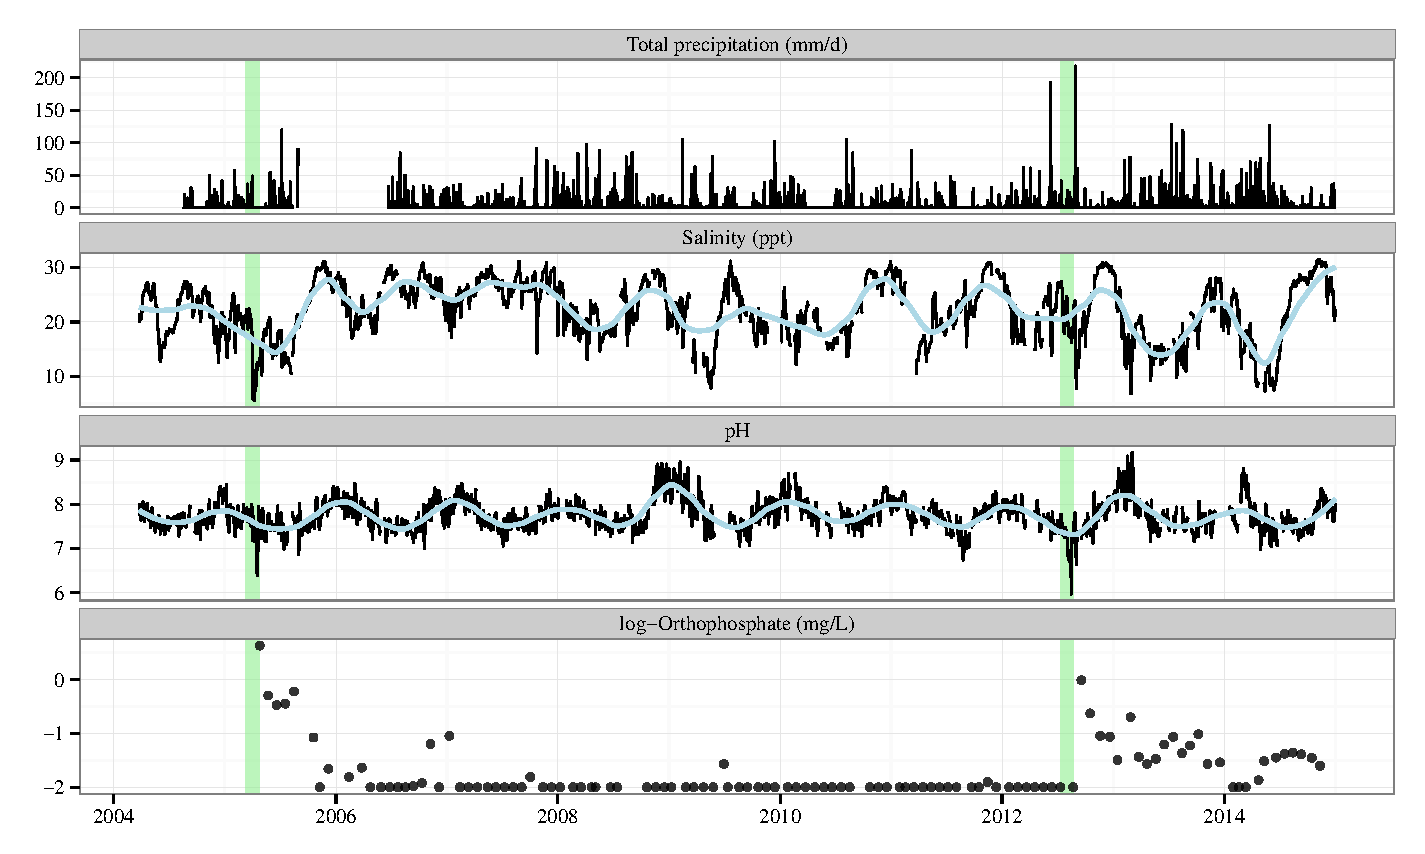
\includegraphics[width=\maxwidth,height=5in]{figs/tsplot-1} 

}

\caption[Time series of total precipitation, salinity, pH, and phosphate for Bangs Lake, Grand Bay reserve]{Time series of total precipitation, salinity, pH, and phosphate for Bangs Lake, Grand Bay reserve.  Vertical green bars indicate a heavy rain event in April 2005 and hurricane Isaac in August 2012.  Salinity and pH include a loess smooth to reduce variability. Orthophosphate is colored by event categories in relation to the vertical green bars.  E1A: event 1 acute, E1C: event 1 chronic, NI: non-impact, E2A: event 2 acute, E2C: event 2 chronic.}\label{fig:tsplot}
\end{figure}


\end{landscape}
\clearpage

\begin{figure}[!ht]

{\centering 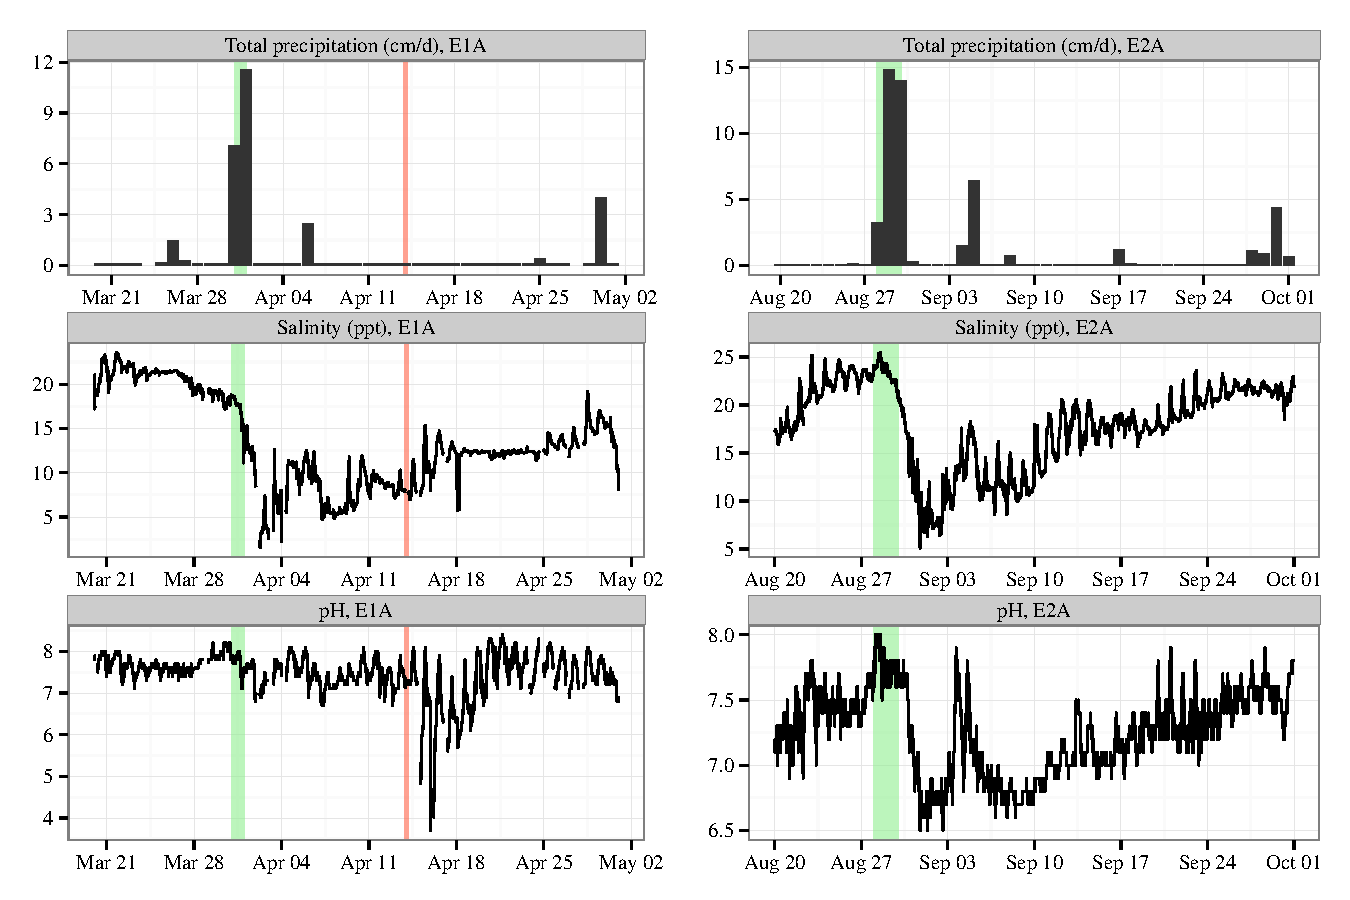
\includegraphics[width=\maxwidth]{figs/tsplotexp-1} 

}

\caption[Time series of total precipitation, salinity, and pH for Bangs Lake, Grand Bay reserve]{Time series of total precipitation, salinity, and pH for Bangs Lake, Grand Bay reserve.  Plots show six month windows centered (green line) around a heavy rain event in April 2005 and hurricane Isaac in August 2012.  E1A: event 1 acute, E2A: event 2 acute.}\label{fig:tsplotexp}
\end{figure}


\clearpage

\begin{figure}[!ht]

{\centering 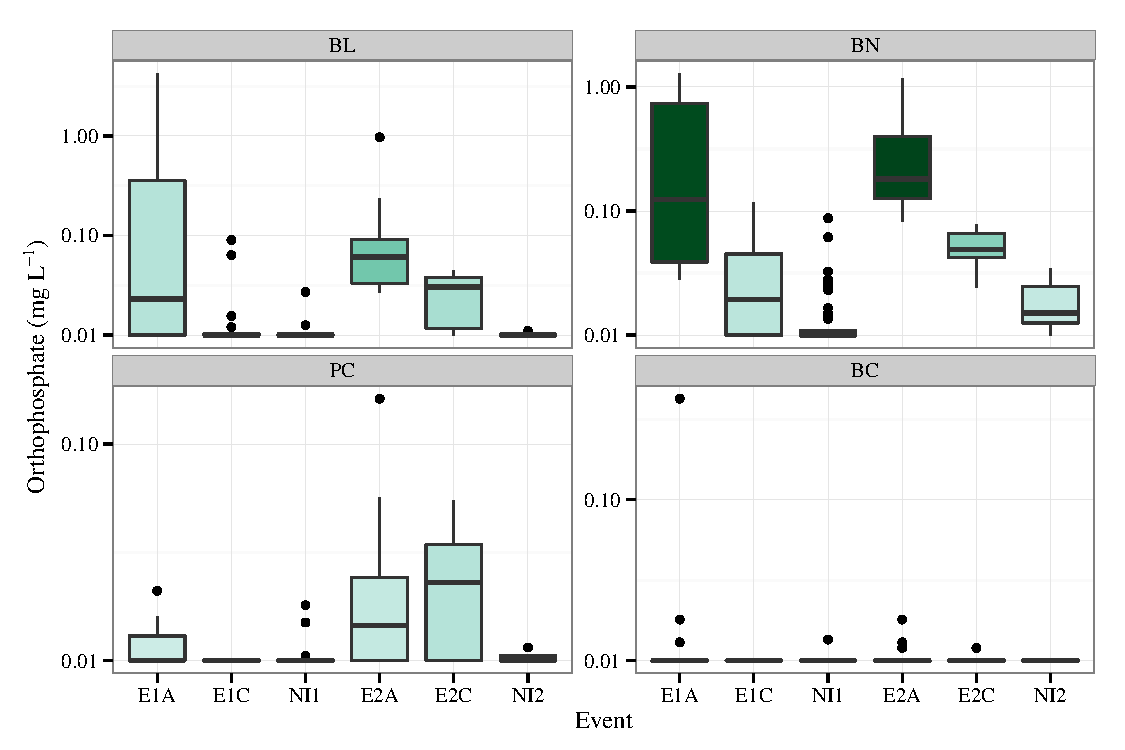
\includegraphics[width=\maxwidth]{figs/orthfig-1} 

}

\caption[Boxplot summaries by event of monthly orthophosphate data at Bangs Lake (BL), and Point aux Chenes (PC), and Bayou Cumbest (BC) sites in Grand Bay]{Boxplot summaries by event of monthly orthophosphate data at Bangs Lake (BL), and Point aux Chenes (PC), and Bayou Cumbest (BC) sites in Grand Bay.  Boxes represent the interquartile range (IQR, 25\textsuperscript{th} to 75\textsuperscript{th} percentile) with the median as the middle horizonal line.  Outliers are present beyond whiskers (1.5$\cdot$IQR). Boxes are shaded by medians between sites.  E1A: event 1 acute, E1C: event 1 chronic, NI: non-impact, E2A: event 2 acute, E2C: event 2 chronic.}\label{fig:orthfig}
\end{figure}


\clearpage

%latex.default(tab, file = "", rowlabel = "Site", caption = cap,     caption.loc = "top", rgroup = unique(res$StationCode), n.rgroup = rep(5,         3), rowname = rows, colheads = c("Result", "Mean", "St. Dev.",         "n", "Min", "Max"), label = "tab:orthtab")%
\begin{table}[!tbp]
\caption{Summaries by site and event of monthly orthophosphate data at Bayou Cumbest (BC), Bangs Lake (BL), and Point aux Chenes (PC) in Grand Bay.  Values are within-group summaries of mean, standard deviation, sample size, and range for orthophosphate by station and time frame.  Result letters indicate time frames within each station that were were not significantly different based on Tukey multiple comparison analyses ($\alpha = 0.05$, corrected to reduce Type I error rates). Timeframes are E1A: event 1 acute, E1C: event 1 chronic, NI: non-impact, E2A: event 2 acute, E2C: event 2 chronic.\label{tab:orthtab}} 
\begin{center}
\begin{tabular}{llrrrrr}
\hline\hline
\multicolumn{1}{l}{Site}&\multicolumn{1}{c}{Result}&\multicolumn{1}{c}{Mean}&\multicolumn{1}{c}{St. Dev.}&\multicolumn{1}{c}{n}&\multicolumn{1}{c}{Min}&\multicolumn{1}{c}{Max}\tabularnewline
\hline
{\bfseries BL}&&&&&&\tabularnewline
~~E1A&a&$-1.15$&$0.89$&$13$&$-2.00$&$ 0.63$\tabularnewline
~~E1C&bc&$-1.89$&$0.28$&$19$&$-2.00$&$-1.05$\tabularnewline
~~NI&c&$-1.99$&$0.06$&$52$&$-2.00$&$-1.57$\tabularnewline
~~E2A&a&$-1.15$&$0.42$&$16$&$-1.57$&$-0.01$\tabularnewline
~~E2C&b&$-1.64$&$0.27$&$11$&$-2.00$&$-1.36$\tabularnewline
\hline
{\bfseries PC}&&&&&&\tabularnewline
~~E1A&bc&$-1.92$&$0.12$&$ 9$&$-2.00$&$-1.68$\tabularnewline
~~E1C&c&$-2.00$&$0.00$&$18$&$-2.00$&$-2.00$\tabularnewline
~~NI&c&$-1.99$&$0.04$&$52$&$-2.00$&$-1.74$\tabularnewline
~~E2A&ab&$-1.73$&$0.35$&$15$&$-2.00$&$-0.79$\tabularnewline
~~E2C&a&$-1.69$&$0.28$&$11$&$-2.00$&$-1.26$\tabularnewline
\hline
{\bfseries BC}&&&&&&\tabularnewline
~~E1A&a&$-1.85$&$0.45$&$13$&$-2.00$&$-0.37$\tabularnewline
~~E1C&b&$-2.00$&$0.00$&$19$&$-2.00$&$-2.00$\tabularnewline
~~NI&b&$-2.00$&$0.02$&$52$&$-2.00$&$-1.87$\tabularnewline
~~E2A&ab&$-1.97$&$0.07$&$16$&$-2.00$&$-1.74$\tabularnewline
~~E2C&ab&$-1.99$&$0.02$&$11$&$-2.00$&$-1.92$\tabularnewline
\hline
\end{tabular}\end{center}

\end{table}

\clearpage


% Table created by stargazer v.5.1 by Marek Hlavac, Harvard University. E-mail: hlavac at fas.harvard.edu
% Date and time: Fri, Jul 10, 2015 - 1:35:28 PM
\begin{table}[!htbp] \centering 
  \caption{Results for generalized least squares models of pH as a function of salinity and station, including interactions.  The constant value is the intercept term defined as mean salinity at Bayou Cumbust (BC) with all other coefficients describing the change in ph from the intercept in relation to each fixed parameter.  One model was created for each time frame.  A first-order autoregressive structure conditional on station was used to account for time-dependent correlation among model residuals.} 
  \label{} 
\begin{tabular}{@{\extracolsep{5pt}}lccc} 
\\[-1.8ex]\hline 
\hline \\[-1.8ex] 
 & \multicolumn{3}{c}{\textit{Dependent variable:}} \\ 
\cline{2-4} 
\\[-1.8ex] & \multicolumn{3}{c}{ph} \\ 
 & E1A & NI & E2A \\ 
\\[-1.8ex] & (1) & (2) & (3)\\ 
\hline \\[-1.8ex] 
 sal & 0.057$^{***}$ & 0.047$^{***}$ & 0.053$^{***}$ \\ 
  & (0.002) & (0.001) & (0.003) \\ 
  & & & \\ 
 StationBL & 0.629$^{***}$ & 0.578$^{***}$ & 0.290 \\ 
  & (0.130) & (0.096) & (0.187) \\ 
  & & & \\ 
 StationPC & 1.931$^{***}$ & 0.607$^{***}$ & 0.917$^{***}$ \\ 
  & (0.172) & (0.091) & (0.164) \\ 
  & & & \\ 
 sal:StationBL & $-$0.017$^{***}$ & $-$0.016$^{***}$ & $-$0.007 \\ 
  & (0.005) & (0.003) & (0.007) \\ 
  & & & \\ 
 sal:StationPC & $-$0.059$^{***}$ & $-$0.011$^{***}$ & $-$0.028$^{***}$ \\ 
  & (0.006) & (0.002) & (0.005) \\ 
  & & & \\ 
 Constant & 6.199$^{***}$ & 6.522$^{***}$ & 6.479$^{***}$ \\ 
  & (0.070) & (0.060) & (0.110) \\ 
  & & & \\ 
\hline \\[-1.8ex] 
Observations & 1,983 & 4,937 & 1,556 \\ 
Log Likelihood & 1,471.083 & 2,944.468 & 705.973 \\ 
Akaike Inf. Crit. & $-$2,926.167 & $-$5,872.935 & $-$1,395.947 \\ 
Bayesian Inf. Crit. & $-$2,881.452 & $-$5,820.909 & $-$1,353.179 \\ 
\hline 
\hline \\[-1.8ex] 
\textit{Note:}  & \multicolumn{3}{r}{$^{*}$p$<$0.1; $^{**}$p$<$0.05; $^{***}$p$<$0.01} \\ 
\end{tabular} 
\end{table} 

\clearpage

%latex.default(totab, file = "", rowlabel = "Site comparisons",     caption = cap.val, caption.loc = "top", rgroup = rgroups,     n.rgroup = rep(3, 2), cgroup = c("First acute event (E1A)",         "Second acute event (E2A)"), n.cgroup = c(2, 2), rowname = wqres$L1,     label = "tab:ccfwq", insert.bottom = foot.val, col.just = c("r",         "c", "r", "c"))%
\begin{table}[!tbp]
\caption{Results of cross-correlation analyses comparing water quality time series between sites at Grand Bay during the two acute event periods.  Seasonal components of each time series are removed.  Values for pH and salinity (ppt) are the lags in the compared time series between sites at which the maximum correlation was observed.  Negative lags indicate observations were leading at the first site relative to the second, whereas positive lags indicate observations lagged at the first site relative to the second.  One lag is thirty minutes.\label{tab:ccfwq}} 
\begin{center}
\begin{tabular}{lrccrc}
\hline\hline
\multicolumn{1}{l}{\bfseries Site comparisons}&\multicolumn{2}{c}{\bfseries First acute event (E1A)}&\multicolumn{1}{c}{\bfseries }&\multicolumn{2}{c}{\bfseries Second acute event (E2A)}\tabularnewline
\cline{2-3} \cline{5-6}
\multicolumn{1}{l}{}&\multicolumn{1}{c}{Lag}&\multicolumn{1}{c}{Correlation}&\multicolumn{1}{c}{}&\multicolumn{1}{c}{Lag}&\multicolumn{1}{c}{Correlation}\tabularnewline
\hline
{\bfseries pH}&&&&&\tabularnewline
~~BC - BL&$ 1$&$0.54$&&$ 1$&$0.21$\tabularnewline
~~BC - PC&$ 4$&$0.18$&&$-1$&$0.14$\tabularnewline
~~BL - PC&$-1$&$0.48$&&$-2$&$0.40$\tabularnewline
\hline
{\bfseries Salinity}&&&&&\tabularnewline
~~BC - BL&$ 0$&$0.86$&&$ 0$&$0.84$\tabularnewline
~~BC - PC&$ 7$&$0.54$&&$40$&$0.44$\tabularnewline
~~BL - PC&$ 1$&$0.83$&&$40$&$0.64$\tabularnewline
\hline
\end{tabular}\end{center}

\footnotesize BC: Bayou Cumbest, BL: Bangs Lake, PC: Point aux Chenes\end{table}

\clearpage

% appendix boxplots
\begin{figure}[!ht]

{\centering 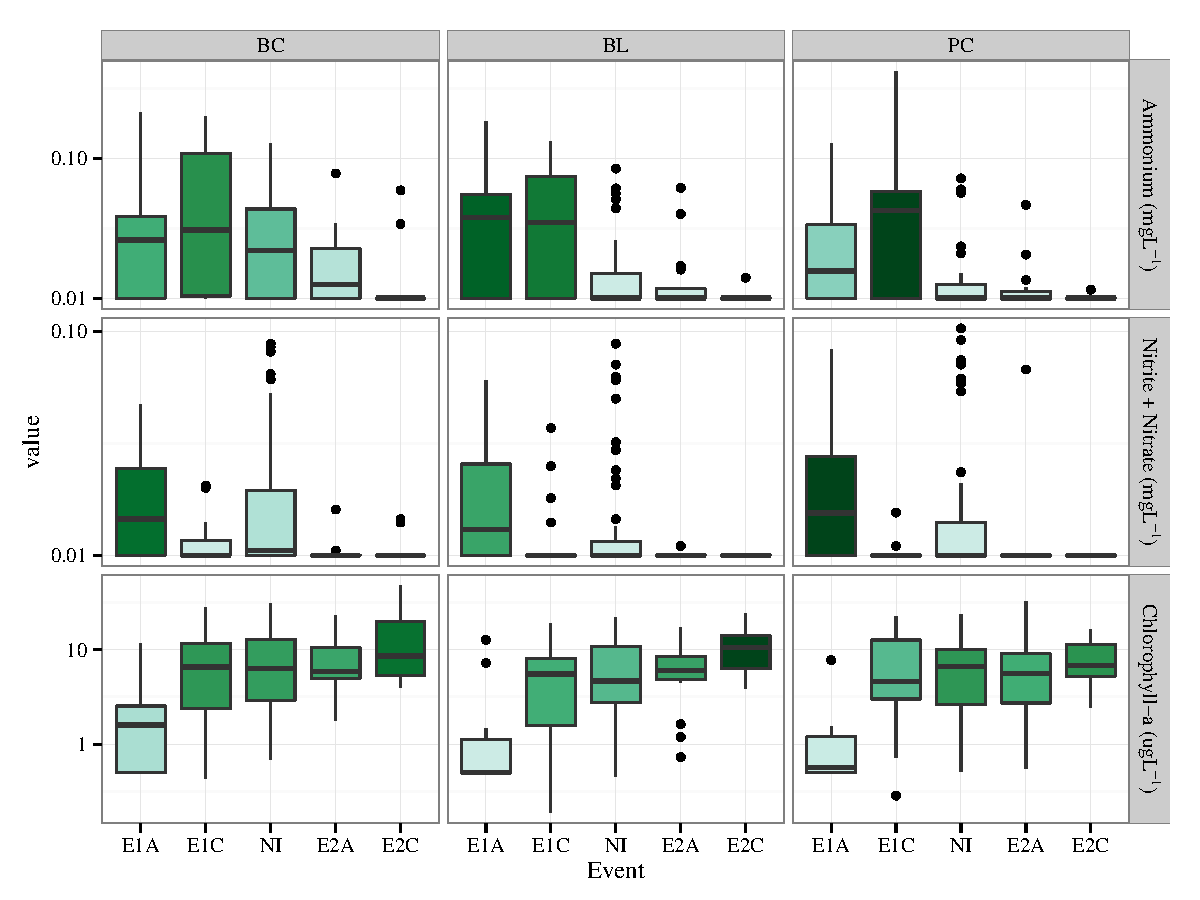
\includegraphics[width=\maxwidth]{figs/boxplt_all-1} 

}

\caption[Boxplot summaries by event of nutrient data at Bayou Cumbest (BC), Bangs Lake (BL), and Point aux Chenes (PC) sites at Grand Bay]{Boxplot summaries by event of nutrient data at Bayou Cumbest (BC), Bangs Lake (BL), and Point aux Chenes (PC) sites at Grand Bay.  Letters indicate significantly different events based on Tukey multiple comparison analyses for each unique site and nutrient value combination.  Boxes represent the interquartile range (IQR, 25\textsuperscript{th} to 75\textsuperscript{th} percentile) with the median as the middle horizonal line.  Boxes are colored by relative median nutrients between sites.  Outliers are present beyond whiskers (1.5$\cdot$IQR). E1A: event 1 acute, E1C: event 1 chronic, NI: non-impact, E2A: event 2 acute, E2C: event 2 chronic.}\label{fig:boxplt_all}
\end{figure}



\end{document}
